\documentclass[../main.tex]{subfiles}
 
\begin{document}

% The asterix after \subsection disables section numbering
\subsection*{Problem 2 Part A}
Determine the combination of ingredients that minimizes calories but meets all nutritional requirements.

\begin{enumerate}[i.]
	\item Formulate the problem as a linear program with an objective function and all constraints.

	We can formulate this problem as the following linear program:

	\begin{equation*}
		\begin{aligned}
			% Minimize calories
			& \text{minimize} & & 21 \cdot w_{\text{tomato}} + 16 \cdot  w_{\text{lettuce}} + 40 \cdot w_{\text{spinach}} + 41 \cdot w_{\text{carrot}} \\
			& & & + 585 \cdot w_{\text{sunflower seed}} + 120 \cdot w_{\text{smoked tofu}} + 164 \cdot w_{\text{chickpea}} + 884 \cdot w_{\text{oil}}\\ \\
			% Subject to >= 15g protein
			& \text{subject to} & & -0.85 \cdot w_{\text{tomato}} - 1.62 \cdot  w_{\text{lettuce}} - 2.86 \cdot w_{\text{spinach}} - 0.93 \cdot w_{\text{carrot}} \\
			& & & - 23.4 \cdot w_{\text{sunflower seed}} - 16 \cdot w_{\text{smoked tofu}} - 9 \cdot w_{\text{chickpea}} - 0 \cdot w_{\text{oil}} \leq -15, \\ \\
			% Subject to >= 2g fat
			& & & - 0.33 \cdot w_{\text{tomato}} - 0.2 \cdot  w_{\text{lettuce}} - 0.39 \cdot w_{\text{spinach}} - 0.24  \cdot w_{\text{carrot}} \\
			& & & - 48.7 \cdot w_{\text{sunflower seed}} - 5 \cdot w_{\text{smoked tofu}} - 2.6 \cdot w_{\text{chickpea}} - 100 \cdot w_{\text{oil}} \leq -2, \\ \\
			% Subject to <= 8g fat
			& & & 0.33 \cdot w_{\text{tomato}} + 0.2 \cdot  w_{\text{lettuce}} + 0.39 \cdot w_{\text{spinach}} + 0.24  \cdot w_{\text{carrot}} \\
			& & & + 48.7 \cdot w_{\text{sunflower seed}} + 5 \cdot w_{\text{smoked tofu}} + 2.6 \cdot w_{\text{chickpea}} + 100 \cdot w_{\text{oil}} \leq 8, \\ \\
			% Subject to >= 4g carbohydrates
			& & & - 4.64 \cdot w_{\text{tomato}} - 2.37 \cdot  w_{\text{lettuce}} - 3.63 \cdot w_{\text{spinach}} - 9.58  \cdot w_{\text{carrot}} \\
			& & & - 15 \cdot w_{\text{sunflower seed}} - 3 \cdot w_{\text{smoked tofu}} - 27 \cdot w_{\text{chickpea}} - 0 \cdot w_{\text{oil}} \leq -4, \\ \\
			% Subject to <= 200 mg sodium
			& & & 9 \cdot w_{\text{tomato}} + 28 \cdot  w_{\text{lettuce}} + 65 \cdot w_{\text{spinach}} + 69  \cdot w_{\text{carrot}} \\
			& & & + 3.8 \cdot w_{\text{sunflower seed}} + 120 \cdot w_{\text{smoked tofu}} + 78 \cdot w_{\text{chickpea}} + 0 \cdot w_{\text{oil}} \leq 200, \\ \\
			% Subject to >= 40% leafy greens by mass
			& & & 0.4 \cdot w_{\text{tomato}} - 0.6 \cdot  w_{\text{lettuce}} - 0.6 \cdot w_{\text{spinach}} + 0.4 \cdot w_{\text{carrot}} \\
			& & & + 0.4 \cdot w_{\text{sunflower seed}} + 0.4 \cdot w_{\text{smoked tofu}} + 0.4 \cdot w_{\text{chickpea}} + 0.4 \cdot w_{\text{oil}} \leq 0, \\ \\
			% Subject to weights greater than or equal to zero
			& & & - w_{\text{tomato}} \leq 0 \\
			& & & - w_{\text{lettuce}} \leq 0 \\
			& & & - w_{\text{spinach}} \leq 0 \\
			& & & - w_{\text{carrot}} \leq 0 \\
			& & & - w_{\text{sunflower seed}} \leq 0 \\
			& & & - w_{\text{smoked tofu}} \leq 0 \\
			& & & - w_{\text{chickpea}} \leq 0 \\
			& & & - w_{\text{oil}} \leq 0 \\
		\end{aligned}
	\end{equation*}

	where the $w$ parameters are the weight of each ingredient, in 100's of grams. The equations, from top to bottom, are:
	\begin{enumerate}[1)]
		\item Minimize total calories
		\item Subject to total protein $\geq$ 15 grams
		\item Subject to total fat $\geq$ 2 grams
		\item Subject to total fat $\leq$ 8 grams
		\item Subject to total carbohydrates $\geq$ 4 grams
		\item Subject to total sodium $\leq$ 200 milligrams
		\item Subject to total leafy green mass $\geq$ 40\% of total mass
		\item Subject to individual ingredient weights $\geq$ 0
	\end{enumerate}

	\item Determine the optimal solution for the linear program using any software you want. Include a copy of the code/file in the report.

	The following MATLAB code was used to generate the solution: \\

	\lstinputlisting{../problem_two/problem2_partA.m}

	where \verb|X| stores the resulting weights of ingredients (in 100's of grams), \verb|FVAL| stores the minimized number of calories, and \verb|EXITFLAG| stores the status of the \verb|linprog| optimization.

	\item What is the cost of the low calorie salad?

	The optimal low calorie salad contains the following weights of ingredients (in 100's of grams):

	\begin{equation*}
		\begin{aligned}
			w_{\text{tomato}} &\approx 0 \\
			w_{\text{lettuce}} &\approx 0.5855 \\
			w_{\text{spinach}} &\approx 0 \\
			w_{\text{carrot}} &\approx 0 \\
			w_{\text{sunflower seed}} &\approx 0 \\
			w_{\text{smoked tofu}} &\approx 0.8782 \\
			w_{\text{chickpea}} &\approx 0 \\
			w_{\text{oil}} &\approx 0 \\
		\end{aligned}
	\end{equation*}

	The optimal low calorie salad costs approximately \$2.33. It contains approximately $114.75$ kcal
\end{enumerate}
\newpage

\subsection*{Problem 2 Part B}
Veronica realizes that it is also important to minimize the cost associated with the new salad. Unfortunately some of the ingredients can be expensive. Determine the combination of ingredients that minimizes cost.

\begin{enumerate}[i.]
	\item Formulate the problem as a linear program with an objective function and all constraints.

	We can formulate this problem as the following linear program:

	\begin{equation*}
		\begin{aligned}
			% Minimize calories
			& \text{minimize} & & 1 \cdot w_{\text{tomato}} + 0.75 \cdot  w_{\text{lettuce}} + 0.5 \cdot w_{\text{spinach}} + 0.5 \cdot w_{\text{carrot}} \\
			& & & + 0.45 \cdot w_{\text{sunflower seed}} + 2.15 \cdot w_{\text{smoked tofu}} + 0.95 \cdot w_{\text{chickpea}} + 2.00 \cdot w_{\text{oil}}\\ \\
			% Subject to >= 15g protein
			& \text{subject to} & & -0.85 \cdot w_{\text{tomato}} - 1.62 \cdot  w_{\text{lettuce}} - 2.86 \cdot w_{\text{spinach}} - 0.93 \cdot w_{\text{carrot}} \\
			& & & - 23.4 \cdot w_{\text{sunflower seed}} - 16 \cdot w_{\text{smoked tofu}} - 9 \cdot w_{\text{chickpea}} - 0 \cdot w_{\text{oil}} \leq -15, \\ \\
			% Subject to >= 2g fat
			& & & - 0.33 \cdot w_{\text{tomato}} - 0.2 \cdot  w_{\text{lettuce}} - 0.39 \cdot w_{\text{spinach}} - 0.24  \cdot w_{\text{carrot}} \\
			& & & - 48.7 \cdot w_{\text{sunflower seed}} - 5 \cdot w_{\text{smoked tofu}} - 2.6 \cdot w_{\text{chickpea}} - 100 \cdot w_{\text{oil}} \leq -2, \\ \\
			% Subject to <= 8g fat
			& & & 0.33 \cdot w_{\text{tomato}} + 0.2 \cdot  w_{\text{lettuce}} + 0.39 \cdot w_{\text{spinach}} + 0.24  \cdot w_{\text{carrot}} \\
			& & & + 48.7 \cdot w_{\text{sunflower seed}} + 5 \cdot w_{\text{smoked tofu}} + 2.6 \cdot w_{\text{chickpea}} + 100 \cdot w_{\text{oil}} \leq 8, \\ \\
			% Subject to >= 4g carbohydrates
			& & & - 4.64 \cdot w_{\text{tomato}} - 2.37 \cdot  w_{\text{lettuce}} - 3.63 \cdot w_{\text{spinach}} - 9.58  \cdot w_{\text{carrot}} \\
			& & & - 15 \cdot w_{\text{sunflower seed}} - 3 \cdot w_{\text{smoked tofu}} - 27 \cdot w_{\text{chickpea}} - 0 \cdot w_{\text{oil}} \leq -4, \\ \\
			% Subject to <= 200 mg sodium
			& & & 9 \cdot w_{\text{tomato}} + 28 \cdot  w_{\text{lettuce}} + 65 \cdot w_{\text{spinach}} + 69  \cdot w_{\text{carrot}} \\
			& & & + 3.8 \cdot w_{\text{sunflower seed}} + 120 \cdot w_{\text{smoked tofu}} + 78 \cdot w_{\text{chickpea}} + 0 \cdot w_{\text{oil}} \leq 200, \\ \\
			% Subject to >= 40% leafy greens by mass
			& & & 0.4 \cdot w_{\text{tomato}} - 0.6 \cdot  w_{\text{lettuce}} - 0.6 \cdot w_{\text{spinach}} + 0.4 \cdot w_{\text{carrot}} \\
			& & & + 0.4 \cdot w_{\text{sunflower seed}} + 0.4 \cdot w_{\text{smoked tofu}} + 0.4 \cdot w_{\text{chickpea}} + 0.4 \cdot w_{\text{oil}} \leq 0, \\ \\
			% Subject to weights greater than or equal to zero
			& & & - w_{\text{tomato}} \leq 0 \\
			& & & - w_{\text{lettuce}} \leq 0 \\
			& & & - w_{\text{spinach}} \leq 0 \\
			& & & - w_{\text{carrot}} \leq 0 \\
			& & & - w_{\text{sunflower seed}} \leq 0 \\
			& & & - w_{\text{smoked tofu}} \leq 0 \\
			& & & - w_{\text{chickpea}} \leq 0 \\
			& & & - w_{\text{oil}} \leq 0 \\
		\end{aligned}
	\end{equation*}

	where the $w$ parameters are the weight of each ingredient, in 100's of grams. The equations, from top to bottom, are:
	\begin{enumerate}[1)]
		\item Minimize total cost
		\item Subject to total protein $\geq$ 15 grams
		\item Subject to total fat $\geq$ 2 grams
		\item Subject to total fat $\leq$ 8 grams
		\item Subject to total carbohydrates $\geq$ 4 grams
		\item Subject to total sodium $\leq$ 200 milligrams
		\item Subject to total leafy green mass $\geq$ 40\% of total mass
		\item Subject to individual ingredient weights $\geq$ 0
	\end{enumerate}

	\item Determine the optimal solution for the linear program using any software you want. Include a copy of the code/file in the report.

	The following MATLAB code was used to generate the solution: \\

	\lstinputlisting{../problem_two/problem2_partB.m}

	where \verb|X| stores the resulting weights of ingredients (in 100's of grams), \verb|FVAL| stores the minimized number of calories, and \verb|EXITFLAG| stores the status of the \verb|linprog| optimization.

	\item How many calories are in the low cost salad?

	The optimal low cost salad contains the following weights of ingredients (in 100's of grams):

	\begin{equation*}
		\begin{aligned}
			w_{\text{tomato}} &\approx 0 \\
			w_{\text{lettuce}} &\approx 0 \\
			w_{\text{spinach}} &\approx 0.8323 \\
			w_{\text{carrot}} &\approx 0 \\
			w_{\text{sunflower seed}} &\approx 0.0961 \\
			w_{\text{smoked tofu}} &\approx 0 \\
			w_{\text{chickpea}} &\approx 1.1524 \\
			w_{\text{oil}} &\approx 0 \\
		\end{aligned}
	\end{equation*}

	The optimal low cost salad costs approximately \$1.55. It contains approximately $278.49$ kcal


\end{enumerate}
\newpage

\subsection*{Problem 2 Part C}
Compare the results from part A and B. Veronica’s goal is to create a Very Veggie Salad that is both low calorie and low cost. She would like to sell the salad for \$5.00 and still have a profit of at least \$3.00. However if she can advertise that the salad has under 250 calories then she may be able to sell more.

\begin{enumerate}[i.]
	\item Suggest some possible ways that she select a combination of ingredients that is “near optimal” for both objectives. This is a type of multi-objective optimization.

	What Veronica should do is attempt to find a ``pareto optimal" solution that accounts for both calories and cost. In order to do this, she should introduce a new parameter $\lambda$ to her optimization formulation. In essence, she would like to:

	\begin{equation*}
		\begin{aligned}
			% Minimize price and calories
			&\text{minimize} & & (1 - \lambda) \cdot \text{CALORIES} + \lambda \cdot \text{PRICE} \\
			&\text{subject to} & & \text{CONSTRAINTS}
		\end{aligned}
	\end{equation*}

	for values of $\lambda$ between 0 and 1. When $\lambda = 0$, she will be finding the minimum calorie combination of ingredients. When $\lambda = 1$, she will be finding the minimum price combination of ingredients. For all values of $\lambda$ inbetween, she will be finding the ``pareto optimal" combination of ingredients. So, she should solve the optimization problem for values of $\lambda$ between 0 and 1. She can then examine these pareto optimal combinations of ingredients to determine which would best meet her goals of \$3.00 profit and under 250 calories. \\

	We can express this as the following linear program:

	\begin{equation*}
		\begin{aligned}
			% Minimize calories
			& \text{minimize} & & (1 - \lambda) \cdot (21 \cdot w_{\text{tomato}} + 16 \cdot  w_{\text{lettuce}} + 40 \cdot w_{\text{spinach}} + 41 \cdot w_{\text{carrot}} \\
			& & & + 585 \cdot w_{\text{sunflower seed}} + 120 \cdot w_{\text{smoked tofu}} + 164 \cdot w_{\text{chickpea}} + 884 \cdot w_{\text{oil}} )\\ 
			& & & + \lambda \cdot (1 \cdot w_{\text{tomato}} + 0.75 \cdot  w_{\text{lettuce}} + 0.5 \cdot w_{\text{spinach}} + 0.5 \cdot w_{\text{carrot}} \\
			& & & + 0.45 \cdot w_{\text{sunflower seed}} + 2.15 \cdot w_{\text{smoked tofu}} + 0.95 \cdot w_{\text{chickpea}} + 2.00 \cdot w_{\text{oil}} )\\ \\
			% Subject to >= 15g protein
			& \text{subject to} & & -0.85 \cdot w_{\text{tomato}} - 1.62 \cdot  w_{\text{lettuce}} - 2.86 \cdot w_{\text{spinach}} - 0.93 \cdot w_{\text{carrot}} \\
			& & & - 23.4 \cdot w_{\text{sunflower seed}} - 16 \cdot w_{\text{smoked tofu}} - 9 \cdot w_{\text{chickpea}} - 0 \cdot w_{\text{oil}} \leq -15, \\ \\
			% Subject to >= 2g fat
			& & & - 0.33 \cdot w_{\text{tomato}} - 0.2 \cdot  w_{\text{lettuce}} - 0.39 \cdot w_{\text{spinach}} - 0.24  \cdot w_{\text{carrot}} \\
			& & & - 48.7 \cdot w_{\text{sunflower seed}} - 5 \cdot w_{\text{smoked tofu}} - 2.6 \cdot w_{\text{chickpea}} - 100 \cdot w_{\text{oil}} \leq -2, \\ \\
			% Subject to <= 8g fat
			& & & 0.33 \cdot w_{\text{tomato}} + 0.2 \cdot  w_{\text{lettuce}} + 0.39 \cdot w_{\text{spinach}} + 0.24  \cdot w_{\text{carrot}} \\
			& & & + 48.7 \cdot w_{\text{sunflower seed}} + 5 \cdot w_{\text{smoked tofu}} + 2.6 \cdot w_{\text{chickpea}} + 100 \cdot w_{\text{oil}} \leq 8, \\ \\
			% Subject to >= 4g carbohydrates
			& & & - 4.64 \cdot w_{\text{tomato}} - 2.37 \cdot  w_{\text{lettuce}} - 3.63 \cdot w_{\text{spinach}} - 9.58  \cdot w_{\text{carrot}} \\
			& & & - 15 \cdot w_{\text{sunflower seed}} - 3 \cdot w_{\text{smoked tofu}} - 27 \cdot w_{\text{chickpea}} - 0 \cdot w_{\text{oil}} \leq -4, \\ \\
			% Subject to <= 200 mg sodium
			& & & 9 \cdot w_{\text{tomato}} + 28 \cdot  w_{\text{lettuce}} + 65 \cdot w_{\text{spinach}} + 69  \cdot w_{\text{carrot}} \\
			& & & + 3.8 \cdot w_{\text{sunflower seed}} + 120 \cdot w_{\text{smoked tofu}} + 78 \cdot w_{\text{chickpea}} + 0 \cdot w_{\text{oil}} \leq 200, \\ \\
			% Subject to >= 40% leafy greens by mass
			& & & 0.4 \cdot w_{\text{tomato}} - 0.6 \cdot  w_{\text{lettuce}} - 0.6 \cdot w_{\text{spinach}} + 0.4 \cdot w_{\text{carrot}} \\
			& & & + 0.4 \cdot w_{\text{sunflower seed}} + 0.4 \cdot w_{\text{smoked tofu}} + 0.4 \cdot w_{\text{chickpea}} + 0.4 \cdot w_{\text{oil}} \leq 0, \\ \\
			% Subject to weights greater than or equal to zero
			& & & - w_{\text{tomato}} \leq 0 \\
			& & & - w_{\text{lettuce}} \leq 0 \\
			& & & - w_{\text{spinach}} \leq 0 \\
			& & & - w_{\text{carrot}} \leq 0 \\
			& & & - w_{\text{sunflower seed}} \leq 0 \\
			& & & - w_{\text{smoked tofu}} \leq 0 \\
			& & & - w_{\text{chickpea}} \leq 0 \\
			& & & - w_{\text{oil}} \leq 0 \\
		\end{aligned}
	\end{equation*}

	\item What combination of ingredient would you suggest and what is the associated cost and calorie.

	Varying $\lambda$ between 0 and 1, and solving the resulting optimization problems, we obtain the following pareto optimal combinations of total calories and total price:

	\begin{center}
		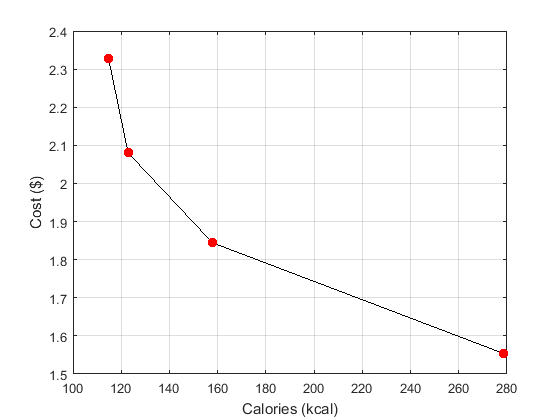
\includegraphics{../problem_two/problem2_partC}
	\end{center}

	Based on this result, I would suggest the following combination of ingredients:

	\begin{equation*}
		\begin{aligned}
			w_{\text{tomato}} &\approx 0 \\
			w_{\text{lettuce}} &\approx 0 \\
			w_{\text{spinach}} &\approx 0.5346 \\
			w_{\text{carrot}} &\approx 0 \\
			w_{\text{sunflower seed}} &\approx 0.0865 \\
			w_{\text{smoked tofu}} &\approx 0.7154 \\
			w_{\text{chickpea}} &\approx 0 \\
			w_{\text{oil}} &\approx 0 \\
		\end{aligned}
	\end{equation*}

	This pareto optimal salad costs approximately \$1.84. It contains approximately $157.86$ kcal. This meets both of Veronicas goals.

	\item Note: There is not one “right” answer. Discuss how you derived your solution.

	The following MATLAB code was used to derive the answer, based on the discussion above.

	\lstinputlisting{../problem_two/problem2_partC.m}


\end{enumerate}

\end{document}